\documentclass{article}\usepackage[]{graphicx}\usepackage[]{color}
%% maxwidth is the original width if it is less than linewidth
%% otherwise use linewidth (to make sure the graphics do not exceed the margin)
\makeatletter
\def\maxwidth{ %
  \ifdim\Gin@nat@width>\linewidth
    \linewidth
  \else
    \Gin@nat@width
  \fi
}
\makeatother

\definecolor{fgcolor}{rgb}{0.345, 0.345, 0.345}
\newcommand{\hlnum}[1]{\textcolor[rgb]{0.686,0.059,0.569}{#1}}%
\newcommand{\hlstr}[1]{\textcolor[rgb]{0.192,0.494,0.8}{#1}}%
\newcommand{\hlcom}[1]{\textcolor[rgb]{0.678,0.584,0.686}{\textit{#1}}}%
\newcommand{\hlopt}[1]{\textcolor[rgb]{0,0,0}{#1}}%
\newcommand{\hlstd}[1]{\textcolor[rgb]{0.345,0.345,0.345}{#1}}%
\newcommand{\hlkwa}[1]{\textcolor[rgb]{0.161,0.373,0.58}{\textbf{#1}}}%
\newcommand{\hlkwb}[1]{\textcolor[rgb]{0.69,0.353,0.396}{#1}}%
\newcommand{\hlkwc}[1]{\textcolor[rgb]{0.333,0.667,0.333}{#1}}%
\newcommand{\hlkwd}[1]{\textcolor[rgb]{0.737,0.353,0.396}{\textbf{#1}}}%

\usepackage{framed}
\makeatletter
\newenvironment{kframe}{%
 \def\at@end@of@kframe{}%
 \ifinner\ifhmode%
  \def\at@end@of@kframe{\end{minipage}}%
  \begin{minipage}{\columnwidth}%
 \fi\fi%
 \def\FrameCommand##1{\hskip\@totalleftmargin \hskip-\fboxsep
 \colorbox{shadecolor}{##1}\hskip-\fboxsep
     % There is no \\@totalrightmargin, so:
     \hskip-\linewidth \hskip-\@totalleftmargin \hskip\columnwidth}%
 \MakeFramed {\advance\hsize-\width
   \@totalleftmargin\z@ \linewidth\hsize
   \@setminipage}}%
 {\par\unskip\endMakeFramed%
 \at@end@of@kframe}
\makeatother

\definecolor{shadecolor}{rgb}{.97, .97, .97}
\definecolor{messagecolor}{rgb}{0, 0, 0}
\definecolor{warningcolor}{rgb}{1, 0, 1}
\definecolor{errorcolor}{rgb}{1, 0, 0}
\newenvironment{knitrout}{}{} % an empty environment to be redefined in TeX

\usepackage{alltt}
\usepackage[margin=0.75in]{geometry}
\usepackage{amsmath,amssymb}
\usepackage{graphicx,float}
\usepackage{multirow,setspace}
\usepackage{enumerate}
\usepackage{booktabs}
\usepackage{placeins}
\usepackage{cite}
\usepackage{caption}
\usepackage{subcaption}
\usepackage{wrapfig}
\usepackage{hyperref}
\usepackage{listings}

\newcommand{\HRule}{\rule{\linewidth}{0.5mm}}
\newcommand{\tab}{\hspace{0.5cm}}
\newcommand{\modref}[1]{(\ref{#1})}
\mathchardef\mhyphen="2D




\newcounter{DefnCounter}
\setcounter{DefnCounter}{1}

\newcounter{ThmCounter}
\setcounter{ThmCounter}{1}

\newcounter{ExampleCounter}
\setcounter{ExampleCounter}{1}

\newcommand{\defn}[1]{\textsc{Definition 1.\arabic{DefnCounter}\stepcounter{DefnCounter}: #1\\} }
\newcommand{\thm}{\textsc{Theorem 1.\arabic{ThmCounter}\stepcounter{ThmCounter}\\} }
\newcommand{\ex}{\textsc{Example 1.\arabic{ExampleCounter}\stepcounter{ExampleCounter}\\} }

\newcommand{\Defn}{\underline{Definition}}
\newcommand{\Q}{\underline{Question}}
\newcommand{\Qs}{\underline{Questions}}
\newcommand{\bbeta}{{\mbox{\boldmath$\beta$}}}
\newcommand{\bmu}{{\mbox{\boldmath$\mu$}}}
\newcommand{\balpha}{{\mbox{\boldmath$\alpha$}}}
\newcommand{\btheta}{{\mbox{\boldmath$\theta$}}}
\newcommand{\bphi}{{\mbox{\boldmath$\phi$}}}
\newcommand{\bSigma}{{\mbox{\boldmath$\Sigma$}}}
\newcommand{\bLambda}{{\mbox{\boldmath$\Lambda$}}}
\newcommand{\bpi}{{\mbox{\boldmath$\pi$}}}
\newcommand{\R}{\texttt{R}}
\newcommand{\Lik}{\mathcal{L}}
\newcommand{\bx}{\textbf{x}}
\newcommand{\by}{\textbf{y}}
\newcommand{\bX}{\textbf{X}}
\newcommand{\sic}{\text{Inv-}\chi^2}


\newcommand{\sao}{SaO$_2$}

\setlength{\marginparwidth}{2cm}
\IfFileExists{upquote.sty}{\usepackage{upquote}}{}
\begin{document}


\begin{center}
	\vspace{0.1cm}
	\textsc{\LARGE MATH 640 Final Project} \\[0.1cm]
	Jason Michaels (jam521), Niko Paulson (ndp32), Miranda Seitz-McLeese (mgs85) 
\end{center}
\section{Introduction}
\label{s:intro}
This analysis will be done on a data set of a variety of measurements about severe weather in the United States. 
The data set contains a variety of measures from severe weather events in the United States from 1996-2016. It was taken from the NOAA website \cite{dataset}.
For this project we focused on the deaths directly attributable to the event.
Understanding how and at what rate severe weather events become lethal in the United States has tremendous public health impacts.
In this paper we compare four possible models for the deaths: The traditional Poisson and negative binomial distributions, as well as the zero inflated variant of each.

The remainder of this analysis is organized as follows: Section~\ref{s:methods} discusses and derives the models. Section~\ref{s:results} describes the results of the analysis. And Section~\ref{s:discussion} contains the conclusions.

\section{Methods}
\label{s:methods}
The deaths attributed to a severe weather event is `count' data. 
The most common model used for count data is the Poisson distribution. 
However for some weather events, the negative binomial model is a better fit, because the Poisson distribution assumes that the events being counted occur independently.

Fortunately, the vast majority of severe weather events in the United States involve no deaths, therefore we wanted to also account for the possibility of structural zeros, therefore we also considered zero inflated variants. 
These distributions are created by returning $0$ with probability $\sigma$ and sampling from the original distribution with probability $(1-\sigma)$. 

We will derive and fit a model for each of the four distributions and see if there is a difference in our results and evaluate to determine which model best fits the data.

\subsection{Poisson}
\label{ss:mPoisson}

\subsection{Negative Binomial}
\label{ss:mNBinom}


\subsection{Zero Inflated Poisson}
\label{ss:mZiPoisson}
The Zero Inflated Poisson (ZIP) model has two parameters. The parameter p is the probability of a structural zero, and $\lambda$ corresponds to the parameter in a typical Poisson model. For a single observation x, the probability density is:

\[
p(x|p, \lambda) = pI_{x=0}(x) + (1-p)\frac{e^{-\lambda}\lambda^x}{x!}
\]


\noindent We can write the likelihood as follows:
$$
L(p, \lambda|X) = \prod_{x_i=0}\bigg[p+(1-p)\frac{e^{-\lambda}\lambda^{x_i}}{x_i!}\bigg]\prod_{x_i \ne 0}\bigg[(1-p)\frac{e^{-\lambda}\lambda^{x_i}}{x_i!}\bigg]
$$

\noindent Bayarri, Berger, and Datta (2008) \cite{ZIP} suggest using the prior distribution $\pi(\lambda, p) \propto \frac{1}{\sqrt{\lambda}}I(0<p<1)$. This gives us the following posterior 

\[
\prod_{x_i=0}\bigg[p+(1-p)\frac{e^{-\lambda}\lambda^{x_i}}{x_i!}\bigg]\prod_{x_i \ne 0}\bigg[(1-p)\frac{e^{-\lambda}\lambda^{x_i - 1/2}}{x_i!}\bigg]
\]

\noindent In obtaining our full conditionals, we can simplify this slightly to obtain the following:

\[
p(\lambda|X, p) \propto \prod_{x_i=0}\bigg[p+(1-p)\frac{e^{-\lambda}\lambda^{x_i}}{x_i!}\bigg]\prod_{x_i \ne 0}\bigg[e^{-\lambda}\lambda^{x_i - 1/2}\bigg]
\]

\[
p(p|X, \lambda) \propto \prod_{x_i=0}\bigg[p+(1-p)\frac{e^{-\lambda}\lambda^{x_i}}{x_i!}\bigg]\prod_{x_i \ne 0}\bigg[(1-p)\bigg]
\]

\noindent Neither of these distributions is recognizable. We can use a Metropolis-Hastings algorithm to sample from both of them. We will use a beta distribution as a proposal for p, and a gamma for $\lambda$. We will tune them to obtain a better acceptance rate. 

\subsection{Zero Inflated Negative Binomial}
\label{ss:mZiNBinom}
The Zero Inflated Negative Binomial (ZINB) model has three parameters $\sigma,$ the probability of a structural zero, and $p,r$ the usual negative binomial parameters. 
For a single $X$ the probability density is: 
$$p(X|\sigma, p, r) = \sigma I_{X=0}(X) + (1-\sigma)\frac{\Gamma(r+X)}{\Gamma(r)X!}.$$
We take the uniform priors for $\sigma$ and $p$ as well as the non-informative gamma for $r$ which is $r^{-1/2}$. For a full derivation, see \ref{a:dZINB}. My posterior is:
$$p(r,\sigma, p|X)\propto\left(\sigma + (1-\sigma)(1-p)^r\right)^Z(1-\sigma)^{N-Z}(1-p)^{(N-Z)r}p^{\sum_{i=1}^NX_i}r^{-1/2}\prod_{i=1}^N\left(\frac{\Gamma(r+X_i)}{\Gamma(r)}\right)$$
This distribution does not factor nicely, so I will use the Metropolis algorithm to sample from it. 
Because this posterior does not suggest any obvious proposal distributions I will sample each independently from a normal distribution centered at $\theta^*$, and with a variance that is tuned to yeild an appropriate acceptance rate.

\section{Results}
\label{s:results}
\subsection{Poisson}
\label{ss:rPoisson}

\subsection{Negative Binomial}
\label{ss:rNBinom}

\subsection{Zero Inflated Poisson}
\label{ss:rZiPoisson}

\subsection{Zero Inflated Negative Binomial}
\label{ss:rZiNBinom}



The ZINB model was fit using the Metropolis-Hastings algorithm with a multivariate truncated normal distribution used as the proposal distribution. For the source code of the sampler, please see \ref{a:cZINB}.

This model suffered severely from the curse of dimensionality. It was very slow to converge, and the very small variance (necessary to tune the acceptance rate) led to high autocorrelation, meaning agressive thinning was necessary. Autocorrelation and running mean plots for both the Tornado and the Flash Flood models can be found in Figure~\ref{f:zinbconvergence}. 


In the end $650000$ samples were drawn originally for each model, with a burn in of $20000$ and one of every $70$ samples was retained, resulting in a final sample size of $9000$. The flood model had an acceptance rate of $0.193$ and the tornado model had an acceptance rate of $0.193$. The resulting densities are pictured in Figure~\ref{f:zinbdensity}, and Table~\ref{t:ZINBparams}, though due to autocorrelation and questions of convergence the results should viewed with caution.



The DIC for floods and tornadoes respectively were $10804$ and $7166$. I was unable to calculate WIACs because it was too computationally expensive.
\begin{table}
\centering
\caption{The following table shows the results of the flash flood ZINB model and the tornado ZINB model. It shows the mean and the median for each parameter as well as the 95\% credible interval.}
\label{t:ZINBparams}
\begin{tabular}{lcccccc}
\toprule
&\multicolumn{3}{c}{Flash Flood}&\multicolumn{3}{c}{Tornado}\\
\cmidrule(r){2-4}\cmidrule(l){5-7}
Parameter & Mean Value &Median Value & (95\% CI)& Mean Value &Median Value & (95\% CI)\\
\midrule
$\sigma$ & 0.305 &
  0.285&
  (0.014, 
    0.712)&
  0.29 &
  0.267&
  (0.012, 
    0.682)\\
$p$ &  0.555 &
  0.555&
  (0.519, 
    0.591)&
  0.862 &
  0.863&
  (0.841, 
    0.882)\\
$r$ &  0.023 &
  0.02&
  (0.014, 
    0.052)&
  0.015 &
  0.013&
  (0.009, 
    0.03)\\
\bottomrule
\end{tabular}
\end{table}
\begin{figure}
	\centering
\begin{knitrout}
\definecolor{shadecolor}{rgb}{0.969, 0.969, 0.969}\color{fgcolor}
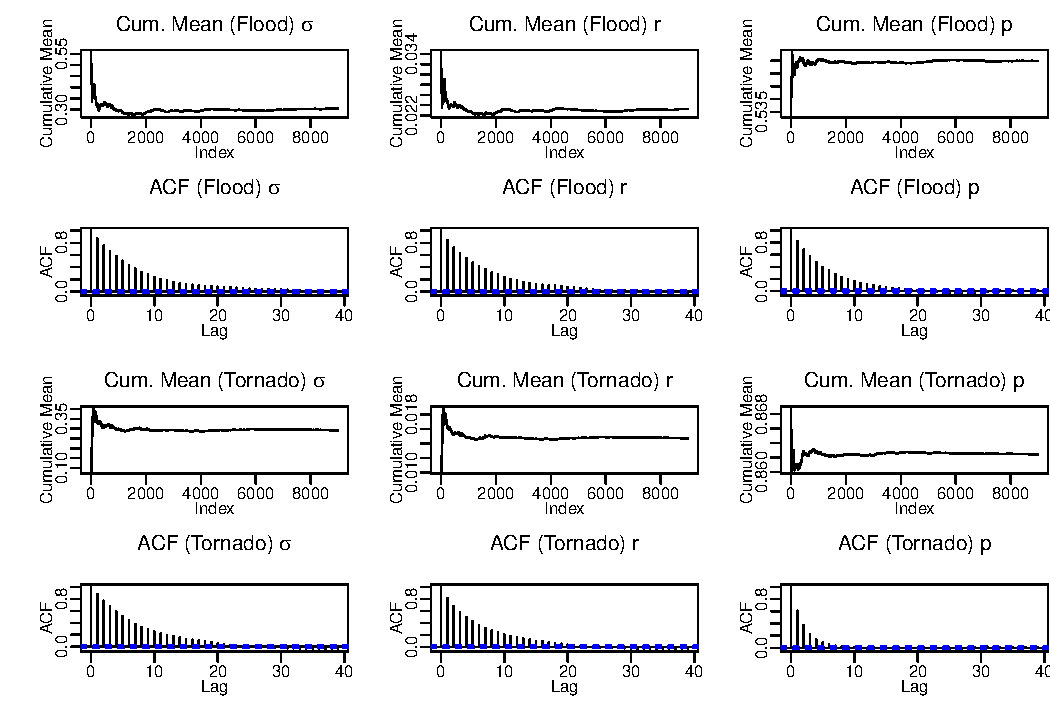
\includegraphics[width=\maxwidth]{figure/floodconvergence-1} 

\end{knitrout}
	\caption{Autocorrelation plots, index plots, and cumulative mean plots for each of the three parameters in the ZINB model fit on flash flood and the tornado data.}
	\label{f:zinbconvergence}
\end{figure} 

\begin{figure}
	\centering
\begin{knitrout}
\definecolor{shadecolor}{rgb}{0.969, 0.969, 0.969}\color{fgcolor}
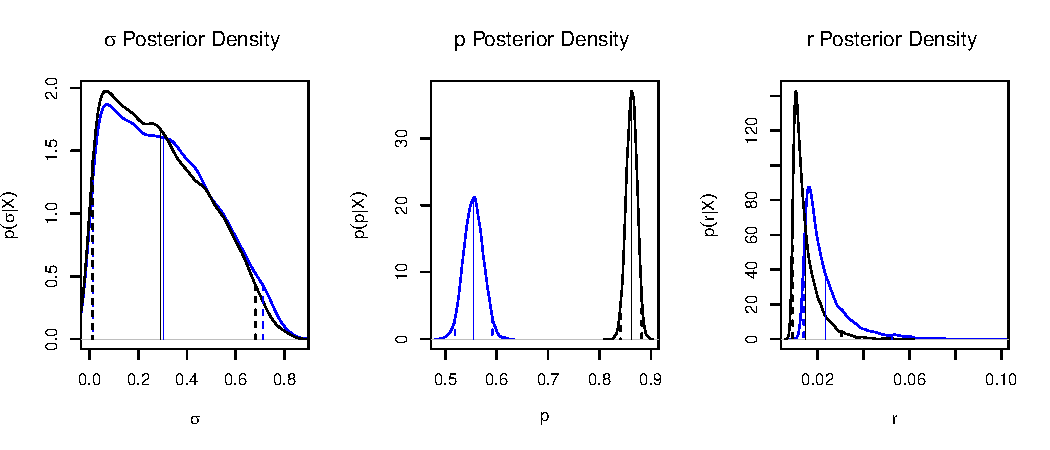
\includegraphics[width=\maxwidth]{figure/zinbdensity-1} 

\end{knitrout}
	\caption{Posterior density curves for each of the three variables. The flood posterior is shown in blue and the tornado posterior is shown in black.}
	\label{f:zinbdensity}
\end{figure} 
\section{Discussion}
\label{s:discussion}

\begin{thebibliography}{2}
  \bibitem{dataset} NOAA's Severe Weather Data Inventory, 
    \url{https://www1.ncdc.noaa.gov/pub/data/swdi/stormevents/csvfiles/}. 
    Accessed April 2017.
  \bibitem{ZIP} Bayarri, M., Berger, J., Datta, G. (2008). Objective testing of Poisson versus inflated Poisson models. IMS 	Collections, 3, 105-121. 
\end{thebibliography}
\clearpage
\appendix
\section{Code}
\label{a:code}
This appendix includes the code used to implement the models.
\subsection{Zero Inflated Negative Binomial code}
\label{a:cZINB}
\begin{knitrout}
\definecolor{shadecolor}{rgb}{0.969, 0.969, 0.969}\color{fgcolor}\begin{kframe}
\begin{alltt}
\hlstd{logpost} \hlkwb{<-} \hlkwa{function}\hlstd{(}\hlkwc{sigma}\hlstd{,} \hlkwc{p}\hlstd{,} \hlkwc{r}\hlstd{,} \hlkwc{Z}\hlstd{,} \hlkwc{N}\hlstd{,} \hlkwc{S}\hlstd{,} \hlkwc{nonzero}\hlstd{)\{}
  \hlstd{lp} \hlkwb{<-} \hlstd{Z}\hlopt{*}\hlkwd{log}\hlstd{(}\hlnum{1} \hlopt{+} \hlstd{(}\hlnum{1}\hlopt{/}\hlstd{sigma}\hlopt{-}\hlnum{1}\hlstd{)}\hlopt{*}\hlstd{(}\hlnum{1}\hlopt{-}\hlstd{p)}\hlopt{^}\hlstd{r)}
  \hlstd{lp} \hlkwb{<-} \hlstd{lp} \hlopt{+} \hlstd{Z}\hlopt{*}\hlkwd{log}\hlstd{(sigma)}
  \hlstd{lp} \hlkwb{<-} \hlstd{lp} \hlopt{+} \hlstd{(N}\hlopt{-}\hlstd{Z)}\hlopt{*}\hlkwd{log}\hlstd{(}\hlnum{1}\hlopt{-}\hlstd{sigma)}
  \hlstd{lp} \hlkwb{<-} \hlstd{lp} \hlopt{+} \hlstd{(N}\hlopt{-}\hlstd{Z)}\hlopt{*}\hlstd{r}\hlopt{*}\hlkwd{log}\hlstd{(}\hlnum{1}\hlopt{-}\hlstd{p)}
  \hlstd{lp} \hlkwb{<-} \hlstd{lp} \hlopt{+} \hlstd{S}\hlopt{*}\hlkwd{log}\hlstd{(p)}
  \hlstd{lp} \hlkwb{<-} \hlstd{lp} \hlopt{-} \hlkwd{log}\hlstd{(r)}\hlopt{/}\hlnum{2}
  \hlstd{lp} \hlkwb{<-} \hlstd{lp} \hlopt{-} \hlstd{(N}\hlopt{-}\hlstd{Z)}\hlopt{*}\hlkwd{lgamma}\hlstd{(r)}
  \hlstd{lp} \hlkwb{<-} \hlstd{lp} \hlopt{+} \hlkwd{sum}\hlstd{(}\hlkwd{lgamma}\hlstd{(r}\hlopt{+}\hlstd{nonzero))}
  \hlkwd{return}\hlstd{(lp)}
\hlstd{\}}

\hlstd{loglik} \hlkwb{<-} \hlkwa{function}\hlstd{(}\hlkwc{sigma}\hlstd{,} \hlkwc{p}\hlstd{,} \hlkwc{r}\hlstd{,} \hlkwc{Z}\hlstd{,} \hlkwc{N}\hlstd{,} \hlkwc{S}\hlstd{,} \hlkwc{nonzero}\hlstd{)\{}
  \hlstd{lp} \hlkwb{<-} \hlstd{Z}\hlopt{*}\hlkwd{log}\hlstd{(}\hlnum{1} \hlopt{+} \hlstd{(}\hlnum{1}\hlopt{/}\hlstd{sigma}\hlopt{-}\hlnum{1}\hlstd{)}\hlopt{*}\hlstd{(}\hlnum{1}\hlopt{-}\hlstd{p)}\hlopt{^}\hlstd{r)}
  \hlstd{lp} \hlkwb{<-} \hlstd{lp} \hlopt{+} \hlstd{Z}\hlopt{*}\hlkwd{log}\hlstd{(sigma)}
  \hlstd{lp} \hlkwb{<-} \hlstd{lp} \hlopt{+} \hlstd{(N}\hlopt{-}\hlstd{Z)}\hlopt{*}\hlkwd{log}\hlstd{(}\hlnum{1}\hlopt{-}\hlstd{sigma)}
  \hlstd{lp} \hlkwb{<-} \hlstd{lp} \hlopt{+} \hlstd{(N}\hlopt{-}\hlstd{Z)}\hlopt{*}\hlstd{r}\hlopt{*}\hlkwd{log}\hlstd{(}\hlnum{1}\hlopt{-}\hlstd{p)}
  \hlstd{lp} \hlkwb{<-} \hlstd{lp} \hlopt{+} \hlstd{S}\hlopt{*}\hlkwd{log}\hlstd{(p)}
  \hlstd{lp} \hlkwb{<-} \hlstd{lp} \hlopt{-} \hlkwd{sum}\hlstd{(}\hlkwd{lgamma}\hlstd{(nonzero}\hlopt{+}\hlnum{1}\hlstd{))}
  \hlstd{lp} \hlkwb{<-} \hlstd{lp} \hlopt{-} \hlstd{(N}\hlopt{-}\hlstd{Z)}\hlopt{*}\hlkwd{lgamma}\hlstd{(r)}
  \hlstd{lp} \hlkwb{<-} \hlstd{lp} \hlopt{+} \hlkwd{sum}\hlstd{(}\hlkwd{lgamma}\hlstd{(r}\hlopt{+}\hlstd{nonzero))}
  \hlkwd{return}\hlstd{(lp)}
\hlstd{\}}

\hlstd{g} \hlkwb{<-}\hlkwa{function}\hlstd{(}\hlkwc{sigma}\hlstd{,} \hlkwc{p}\hlstd{,} \hlkwc{r}\hlstd{,}
             \hlkwc{sigma.mean}\hlstd{,} \hlkwc{p.mean}\hlstd{,} \hlkwc{r.mean}\hlstd{,}
             \hlkwc{sigma.var}\hlstd{,} \hlkwc{p.var}\hlstd{,} \hlkwc{r.var}\hlstd{)\{}
    \hlkwd{return}\hlstd{(}\hlkwd{dtruncnorm}\hlstd{(sigma,} \hlnum{0}\hlstd{,} \hlnum{1}\hlstd{, sigma.mean,} \hlkwd{sqrt}\hlstd{(sigma.var))}\hlopt{*}
           \hlkwd{dtruncnorm}\hlstd{(p,} \hlnum{0}\hlstd{,} \hlnum{1}\hlstd{, p.mean,} \hlkwd{sqrt}\hlstd{(p.var))}\hlopt{*}
           \hlkwd{dtruncnorm}\hlstd{(r,} \hlnum{0}\hlstd{,} \hlnum{Inf}\hlstd{, r.mean,} \hlkwd{sqrt}\hlstd{(r.var)))}
\hlstd{\}}


\hlstd{zinb.sampler} \hlkwb{<-} \hlkwa{function}\hlstd{(}\hlkwc{df}\hlstd{,} \hlkwc{event_type}\hlstd{,} \hlkwc{chainlen}\hlstd{,}
                         \hlkwc{r.var}\hlstd{=}\hlnum{1}\hlstd{,} \hlkwc{p.var}\hlstd{=}\hlnum{1}\hlstd{,} \hlkwc{sigma.var}\hlstd{=}\hlnum{1}\hlstd{,}
                         \hlkwc{burnin}\hlstd{=}\hlnum{0}\hlstd{,} \hlkwc{thinning}\hlstd{=}\hlnum{1}\hlstd{)\{}
  \hlstd{X} \hlkwb{<-} \hlstd{df[df}\hlopt{$}\hlstd{EVENT_TYPE}\hlopt{==}\hlstd{event_type,}\hlstr{"DEATHS_DIRECT"}\hlstd{]}
  \hlstd{N} \hlkwb{<-} \hlkwd{length}\hlstd{(X)}
  \hlstd{Z} \hlkwb{<-} \hlkwd{sum}\hlstd{(X}\hlopt{==}\hlnum{0}\hlstd{)}
  \hlstd{S} \hlkwb{<-} \hlkwd{sum}\hlstd{(X)}
  \hlstd{nonzero} \hlkwb{<-} \hlstd{X[X}\hlopt{!=}\hlnum{0}\hlstd{]}
  \hlstd{B} \hlkwb{<-} \hlstd{chainlen}
  \hlstd{b} \hlkwb{<-} \hlstd{burnin}
  \hlstd{r.sd} \hlkwb{<-} \hlkwd{sqrt}\hlstd{(r.var)}
  \hlstd{p.sd} \hlkwb{<-} \hlkwd{sqrt}\hlstd{(p.var)}
  \hlstd{sigma.sd} \hlkwb{<-} \hlkwd{sqrt}\hlstd{(sigma.var)}

  \hlstd{r.array} \hlkwb{<-} \hlkwd{rep}\hlstd{(}\hlnum{0}\hlstd{, B)}
  \hlstd{sigma.array} \hlkwb{<-} \hlkwd{rep}\hlstd{(}\hlnum{0}\hlstd{, B)}
  \hlstd{p.array} \hlkwb{<-} \hlkwd{rep}\hlstd{(}\hlnum{0}\hlstd{, B)}
  \hlstd{ar.array} \hlkwb{<-} \hlkwd{rep}\hlstd{(}\hlnum{0}\hlstd{, B)}
  \hlstd{posts} \hlkwb{<-} \hlkwd{rep}\hlstd{(}\hlnum{0}\hlstd{, B)}

  \hlstd{r.array[}\hlnum{1}\hlstd{]} \hlkwb{<-} \hlnum{.5}
  \hlstd{p.array[}\hlnum{1}\hlstd{]} \hlkwb{<-} \hlkwd{min}\hlstd{(}\hlkwd{mean}\hlstd{(X),} \hlnum{.5}\hlstd{)}
  \hlstd{sigma.array[}\hlnum{1}\hlstd{]} \hlkwb{<-} \hlkwd{mean}\hlstd{(X}\hlopt{==}\hlnum{0}\hlstd{)}\hlopt{/}\hlnum{2}
  \hlcom{#print(c(r.array[1], p.array[1], sigma.array[1]))}
  \hlstd{posts[}\hlnum{1}\hlstd{]} \hlkwb{<-} \hlkwd{logpost}\hlstd{(sigma.array[}\hlnum{1}\hlstd{], p.array[}\hlnum{1}\hlstd{], r.array[}\hlnum{1}\hlstd{], Z, N, S, nonzero)}
  \hlkwa{for}\hlstd{(i} \hlkwa{in} \hlnum{2}\hlopt{:}\hlstd{chainlen)\{}
    \hlstd{sigma.star} \hlkwb{<-} \hlkwd{rtruncnorm}\hlstd{(}\hlnum{1}\hlstd{,} \hlnum{0}\hlstd{,} \hlnum{1}\hlstd{, sigma.array[i}\hlopt{-}\hlnum{1}\hlstd{], sigma.sd)}
    \hlstd{p.star} \hlkwb{<-} \hlkwd{rtruncnorm}\hlstd{(}\hlnum{1}\hlstd{,} \hlnum{0}\hlstd{,} \hlnum{1}\hlstd{, p.array[i}\hlopt{-}\hlnum{1}\hlstd{], p.sd)}
    \hlstd{r.star} \hlkwb{<-} \hlkwd{rtruncnorm}\hlstd{(}\hlnum{1}\hlstd{,} \hlnum{0}\hlstd{,} \hlnum{Inf}\hlstd{, r.array[i}\hlopt{-}\hlnum{1}\hlstd{], r.sd)}
    \hlstd{lpost} \hlkwb{<-}\hlkwd{logpost}\hlstd{(sigma.star, p.star, r.star, Z, N, S, nonzero)}
    \hlstd{reject.prob} \hlkwb{<-} \hlkwd{exp}\hlstd{(lpost}\hlopt{-}\hlstd{posts[i}\hlopt{-}\hlnum{1}\hlstd{])}\hlopt{*}
                   \hlkwd{dtruncnorm}\hlstd{(sigma.array[i}\hlopt{-}\hlnum{1}\hlstd{],} \hlnum{0}\hlstd{,} \hlnum{1}\hlstd{,}
                              \hlstd{sigma.star, sigma.sd)}\hlopt{*}
                   \hlkwd{dtruncnorm}\hlstd{(p.array[i}\hlopt{-}\hlnum{1}\hlstd{],} \hlnum{0}\hlstd{,} \hlnum{1}\hlstd{, p.star, p.sd)}\hlopt{*}
                   \hlkwd{dtruncnorm}\hlstd{(r.array[i}\hlopt{-}\hlnum{1}\hlstd{],} \hlnum{0}\hlstd{,} \hlnum{Inf}\hlstd{, r.star, r.sd)}\hlopt{/}
                  \hlstd{(}\hlkwd{dtruncnorm}\hlstd{(sigma.star,} \hlnum{0}\hlstd{,} \hlnum{1}\hlstd{,}
                              \hlstd{sigma.array[i}\hlopt{-}\hlnum{1}\hlstd{], sigma.sd)}\hlopt{*}
                     \hlkwd{dtruncnorm}\hlstd{(p.star,} \hlnum{0}\hlstd{,} \hlnum{1}\hlstd{, p.array[i}\hlopt{-}\hlnum{1}\hlstd{], p.sd)}\hlopt{*}
                     \hlkwd{dtruncnorm}\hlstd{(r.star,} \hlnum{0}\hlstd{,} \hlnum{Inf}\hlstd{, r.array[i}\hlopt{-}\hlnum{1}\hlstd{], r.sd))}
    \hlstd{u} \hlkwb{<-} \hlkwd{runif}\hlstd{(}\hlnum{1}\hlstd{,}\hlnum{0}\hlstd{,}\hlnum{1}\hlstd{)}
    \hlkwa{if}\hlstd{(u} \hlopt{<} \hlkwd{min}\hlstd{(reject.prob,} \hlnum{1}\hlstd{))\{}
      \hlstd{r.array[i]} \hlkwb{<-} \hlstd{r.star}
      \hlstd{p.array[i]} \hlkwb{<-} \hlstd{p.star}
      \hlstd{sigma.array[i]} \hlkwb{<-} \hlstd{sigma.star}
      \hlstd{ar.array[i]} \hlkwb{<-} \hlnum{1}
      \hlstd{posts[i]} \hlkwb{<-} \hlstd{lpost}
    \hlstd{\}}
    \hlkwa{else}\hlstd{\{}
      \hlstd{r.array[i]} \hlkwb{<-} \hlstd{r.array[i}\hlopt{-}\hlnum{1}\hlstd{]}
      \hlstd{p.array[i]} \hlkwb{<-} \hlstd{p.array[i}\hlopt{-}\hlnum{1}\hlstd{]}
      \hlstd{sigma.array[i]} \hlkwb{<-} \hlstd{sigma.array[i}\hlopt{-}\hlnum{1}\hlstd{]}
      \hlstd{posts[i]} \hlkwb{<-} \hlstd{posts[i}\hlopt{-}\hlnum{1}\hlstd{]}
    \hlstd{\}}
  \hlstd{\}}
  \hlstd{inds} \hlkwb{<-} \hlkwd{seq}\hlstd{(b}\hlopt{+}\hlnum{1}\hlstd{, B,} \hlkwc{by}\hlstd{=thinning)}
  \hlkwd{return}\hlstd{(}\hlkwd{list}\hlstd{(}\hlkwc{sigma}\hlstd{=sigma.array[inds],}
              \hlkwc{p}\hlstd{=p.array[inds],}
              \hlkwc{r}\hlstd{=r.array[inds],}
              \hlkwc{ar}\hlstd{=ar.array))}
\hlstd{\}}
\end{alltt}
\end{kframe}
\end{knitrout}

\section{Derivations}
\label{a:derivation}
This appendix will include details on the calculations required to derive our models.
\subsection{Zero Inflated Negative Binomial Derivation}
\label{a:dZINB}
The likelihood for the ZINB is 
\begin{align*}
\mathcal{L}(X|\sigma, p, r) &= \prod_{i=1}^N \sigma I_{X=0}(X_i) + (1-\sigma)\frac{\Gamma(r+X_i)}{\Gamma(r)X_i!}\\
\intertext{For ease of notation let $Z$ be the number of zero values in $X$, and $N$ be the total number of observations.}
&=\prod_{X_i=0}\left(\sigma + (1-\sigma)p^{X_i}(1-p)^r\frac{\Gamma(r+X_i)}{\Gamma(r)X_i!}\right)\prod_{X_i\ne 0}\left((1-\sigma)p^{X_i}(1-p)^r\frac{\Gamma(r+X_i)}{\Gamma(r)X_i!}\right)\\
&=\left(\sigma + (1-\sigma)(1-p)^r\right)^Z\prod_{X_i\ne 0}\left((1-\sigma)p^{X_i}(1-p)^r\frac{\Gamma(r+X_i)}{\Gamma(r)X_i!}\right)\\
&\propto\left(\sigma + (1-\sigma)(1-p)^r\right)^Z\prod_{X_i\ne 0}\left((1-\sigma)p^{X_i}(1-p)^r\frac{\Gamma(r+X_i)}{\Gamma(r)}\right)\\
&\propto\left(\sigma + (1-\sigma)(1-p)^r\right)^Z(1-\sigma)^{N-Z}(1-p)^{(N-Z)r}p^{\sum_{i=1}^NX_i}\prod_{i=1}^n\left(\frac{\Gamma(r+X_i)}{\Gamma(r)}\right)
\end{align*}
As mentioned in section \ref{ss:mZiNBinom} we take the uniform priors for $\sigma$ and $p$ as well as the non-informative gamma for $r$ which is $r^{-1/2}$. Therefore my joint posterior is:
\begin{align*}
p(r,\sigma, p|X)\propto&\left(\sigma + (1-\sigma)(1-p)^r\right)^Z(1-\sigma)^{N-Z}(1-p)^{(N-Z)r}p^{\sum_{i=1}^NX_i}r^{-1/2}\prod_{i=1}^N\left(\frac{\Gamma(r+X_i)}{\Gamma(r)}\right)\\
\intertext{I am now going to take the log of the posterior because it helps with computation}
\ln\left(p(r,\sigma, p|X)\right)\propto&Z\ln\left(1 + (1/\sigma-1)(1-p)^r\right) + Z\ln(\sigma) + (N-Z)\ln(1-\sigma)+(N-Z)r\ln(1-p)\\
&+\sum_{i=1}^NX_i\ln(p)-\ln(r)/2-N\ln(\Gamma(r))+\sum_{i=1}^N\ln(\Gamma(r+X_i))
\end{align*}
\end{document}
